\subsection{Unterschiede zwischen den Versionen}
% PAL vs NTSC
Ein regionaler Unterschied zwischen den Versionen liegt im Bildübertragungsverfahren. Europäische Versionen des Spiels verwenden das \ac{PAL}-Verfahren und andere Versionen das \ac{NTSC}-Verfahren. Im Vordergrund steht die unterschiedliche Hertz-Anzahl dieser Verfahren.
Dabei unterstützt  \ac{PAL} ein vielfaches von 50 und \ac{NTSC} ein vielfaches von 60 Hertz\cite{pal-vs-ntsc}. Die Hertzangabe ist in diesem Fall ausschlaggebend dafür, wie oft pro Sekunde der Fernseher Einzelbilder rendern kann.\\

% PAL Bug
Aufgrund eines Fehlers in der \ac{PAL}-Version ist es in einigen Ausgaben des Spiels nicht möglich, das Spiel durchzuspielen. Der Fehler verhindert den Zugang zu Ogremons Festung und das Betreiben des Aufzugs im Berg der Unendlichkeit\cite{epicplay}. Beide Inhalte sind elementarer Bestandteil der Story und nötig, um das Spiel durchzuspielen. Die \ac{NTSC}-Version enthält ebenfalls mehrere Fehler, welche zum Einfrieren des Spiels führen können\cite{gamefaqglitch}. Allerdings verhindern diese nicht die Komplettierung des Spiels.\\

\begin{figure}[H]%
    \centering
    \subfloat[\centering Schatten]{{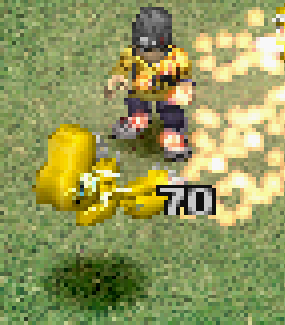
\includegraphics[width=4cm]{figures/screenshots/shadow.png}
    \label{fig:dw1-shadow-a}}}%
    \qquad
    \subfloat[\centering Echtzeitschatten]{{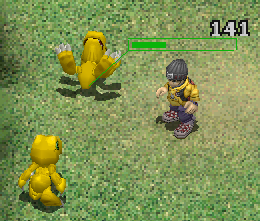
\includegraphics[width=7cm]{figures/screenshots/korean.png} }\label{fig:dw1-shadow-b}}%
    \caption{Unterschiedliche Methodiken zur Schattierung von Objekten}%
    \label{fig:dw1-shadow}%
\end{figure}

% PC Version
Zusätzlich ist das Spiel im April 2002 in Korea für den PC erschienen\cite{korea-multi}. Im Vergleich zu der \ac{PSX}-Version existieren zwei nennenswerte Unterschiede. Zum einen ist es möglich das Spiel an jeder beliebigen Position zu speichern, zum anderen werden Echtzeitschatten von Charakteren gerendert. Dies ist deutlich in \autoref{fig:dw1-shadow-b} zu sehen. Einige Texturen sind ebenfalls hochauflösender.\\

Aufgrund der Tatsache, dass die Verkaufszahlen allerdings nur $\approx 6{,}15\%$ der gesamten Verkaufszahlen ausmachen und einige Unterschiede zu der \ac{PSX}-Version existieren, wird die PC-Version kein zentraler Bestandteil der Untersuchung sein\cite{vgchartz}. Die \ac{PSX}-Spiele wurden zusammen mit einem Handbuch für das Spiel verkauft. Im Anhang der Arbeit befinden sich die Handbücher in japanischer, amerikanischer und deutscher Fassung. Die Handbücher und einige Unterschiede werden im \autoref{sec:game-content} vorgestellt.\\